\floatname{algorithm}{算法}
\renewcommand{\algorithmicrequire}{\textbf{输入：}}
\renewcommand{\algorithmicensure}{\textbf{输出：}}

\section{密码资产识别与量子风险的基本概念}
\label{sec:asset-theory}

\subsection{识别对象与证据层次}

电力终端及其他嵌入式电子设备的密码功能，可能由业务源码、
静态链接代码、动态链接库或独立密码硬件提供。
本方案实现的密码资产扫描工具记为 QCS，
面向 C/C++ 源文件、ELF/PE 程序文件和可提取文件系统的固件镜像，
分别通过词法分析、结构化符号解析、字节特征与已知函数签名获取静态证据。
固件通道将镜像内的程序和库作为组件送入同一检测流程，
使不同输入形式具有一致的算法命名和证据格式。
文本配置中的名称与库依赖也被保留，但其含义需要单独解释。

资产识别至少涉及三个层次：源码或二进制对某算法接口的静态引用、
文件中包含相应实现的静态证据，以及业务运行时实际执行该算法。
接口引用不保证实现位于当前文件；
包含实现也不保证该功能已被启用。
本工具输出前两类证据，运行时使用字段保持未知。
已审查接口的函数定义首先提供命名线索；
当前实现包含预测还要求与固定源码参考的 SHA-256 相符，
或由受限标准运算图给出已实现的依赖见证。
不能仅由函数名证明函数体具有完整、正确的密码语义。
用于评测的实现真值还需独立核对上游源码和构建配置。

当前核心评测集合为 AES、DES、RC4、ChaCha20、RSA、ECDSA、ECDH、
MD5、SHA-1、SHA-256、SM2、SM3 和 SM4，共 13 种。
模型还允许记录其他算法和算法族，
但具体输出范围取决于已审核接口与规则；
类型字典中存在某个名称不等于所有检测通道均已覆盖该算法。
Base64 单独归为编码线索，不能计为密码算法。

本工具在统一调度和证据模型中复用了
Wind River crypto-detector 的文本特征、crypto-detection 的 YARA 规则
及 Binwalk 2 的固件解包能力，
并结合结构化符号检测与自写已知函数识别
\cite{wind-detector,crypto-rules,qryx-detector,binwalk-v2}。
在此基础上，源码角色判定、规则含义映射、
整函数重定位掩码与常量约束、组件溯源及双口径评测
由本项目实现。
依赖版本、规则摘要和参考构建信息随工程保存，
作为判断报告适用范围和复现实验的依据。

共享结构是静态识别必须处理的限制。
SHA-224 与 SHA-256 复用压缩结构，BLAKE2 与 SHA-2 使用同源初始化常量，
ECDSA 与 ECDH 复用椭圆曲线点运算
\cite{rfc6234,rfc7693}。
若证据只支持共享结构，工具将其记录为候选线索，
而不把同一命中展开为多个确定算法。
本章先说明密码算法与量子威胁的理论基础，
再解释上述证据如何在当前实现中产生和组合。

\subsection{基本运算与量子风险}
\label{subsec:basic-quantum-risk}

\paragraph{基本运算与实现差异}
本文以 \(\oplus\) 表示按位异或，
以 \(\land\)、\(\lor\) 和 \(\neg\)
表示按位与、或和取反。
\(\operatorname{ROTL}_w(x,s)\) 与
\(\operatorname{ROTR}_w(x,s)\)
分别表示 \(w\) 位字的循环左移和循环右移；
逻辑右移记为 \(\operatorname{SHR}_w(x,s)\)。
对 \(0<s<w\)，有
\begin{equation}
  \operatorname{ROTL}_w(x,s)
  =
  \bigl((x\ll s)\lor(x\gg(w-s))\bigr)\bmod 2^w.
\end{equation}
同一运算可由不同指令序列实现，
常量也可能因字节序、数据宽度及编译优化而呈现不同形式。
例如，32 位常量 \(\texttt{0x6a09e667}\)
在小端表示中对应 \(\texttt{67 E6 09 6A}\)。
这些实现差异既是构造特征规则的依据，
也是漏报的重要来源。


\paragraph{量子态与测量的必要记号}
以下采用 \(\lvert x\rangle\) 表示编码整数 \(x\) 的计算基态。
量子寄存器的纯态可写为
\begin{equation}
  \lvert\psi\rangle=\sum_x\alpha_x\lvert x\rangle,
  \qquad \sum_x|\alpha_x|^2=1,
\end{equation}
其中 \(\alpha_x\) 为复数幅度；
在计算基下测量得到 \(x\) 的概率为 \(|\alpha_x|^2\)。
量子算法通过可逆运算和干涉改变这些幅度，
最终测量仍只得到一个结果。
因此，均匀叠加不意味着能够一次读出所有候选值；
有效加速需要利用问题结构或设计幅度放大过程
\cite{quantum-revisited,amplitude-amplification}。


\paragraph{Shor 算法：整数分解与量子阶寻找}
Shor 算法能够在理想量子计算模型下，
以输入比特长度的多项式规模求解整数分解和离散对数问题
\cite{shor1997}。
以整数分解为例，先对偶数、素数和素数幂进行经典预处理，
再考虑具有至少两个不同素因子的奇合数 \(N\)。
随机选取 \(a\in\{2,\ldots,N-2\}\)。
若 \(1<\gcd(a,N)<N\)，已获得非平凡因子；
否则，在 \(\gcd(a,N)=1\) 时，定义 \(a\) 模 \(N\) 的阶为
\begin{equation}
  r=\min\{t\geq1:a^t\equiv1\pmod N\}.
  \label{eq:pre-shor-order}
\end{equation}
函数 \(f(x)=a^x\bmod N\) 具有周期 \(r\)，
整数分解由此转化为阶寻找问题。

若 \(r\) 为偶数，且
\(b=a^{r/2}\bmod N\) 不等于 \(1\) 或 \(N-1\)，则
\begin{equation}
  (a^{r/2}-1)(a^{r/2}+1)\equiv0\pmod N,
\end{equation}
从而可以通过
\begin{equation}
  g_-=\gcd(b-1,N),\qquad
  g_+=\gcd(b+1,N)
  \label{eq:pre-shor-factor}
\end{equation}
提取非平凡因子。
求最大公因数和核验因子均为经典计算；
量子部分主要负责获得阶的相关信息。

为说明量子子过程，选取 \(Q=2^t\)，使
\(N^2\leq Q<2N^2\)，
并准备两个寄存器的状态
\begin{equation}
  \lvert\psi_0\rangle
  =\frac{1}{\sqrt Q}\sum_{x=0}^{Q-1}
    \lvert x\rangle\lvert0\rangle.
\end{equation}
可逆模幂电路将其变换为
\begin{equation}
  \lvert\psi_1\rangle
  =\frac{1}{\sqrt Q}\sum_{x=0}^{Q-1}
    \lvert x\rangle\lvert a^x\bmod N\rangle.
  \label{eq:pre-shor-modexp}
\end{equation}
量子傅里叶变换（Quantum Fourier Transform，QFT）定义为
\begin{equation}
  \operatorname{QFT}_Q\lvert x\rangle
  =\frac{1}{\sqrt Q}\sum_{y=0}^{Q-1}
    \exp\left(\frac{2\pi\mathrm{i}xy}{Q}\right)
    \lvert y\rangle,
\end{equation}
其中 \(\mathrm{i}^2=-1\)。
对第一寄存器施加逆 QFT 后测量得到 \(y\)，
其分布在对应于 \(y/Q\) 接近 \(j/r\) 的位置形成峰值，
其中 \(j\in\{0,\ldots,r-1\}\)。
若
\begin{equation}
  \left|\frac{y}{Q}-\frac{j}{r}\right|
  <\frac{1}{2r^2},
  \qquad \gcd(j,r)=1,
  \label{eq:pre-shor-cf}
\end{equation}
则可通过 \(y/Q\) 的连分数展开恢复分母 \(r\)。
测量并非每次都满足这些条件；
若 \(j\) 与 \(r\) 不互素，约分后的分母可能只给出阶的因子。
因此，候选分母需要经过模幂检验，
并根据结果重采样或采用进一步的经典后处理
\cite{shor1997,quantum-revisited}。

算法~\ref{alg:pre-shor-factor} 给出保留失败重试的分解流程，
其中列出了量子态制备、可逆模幂、傅里叶采样和经典后处理。
未获得通过检验的候选时，
将本次阶寻找结果标记为 \(\bot\)，继续下一次尝试。
检验 \(a^r\equiv1\pmod N\) 只能确认候选是一个周期，
并不单独证明其为最小正周期，
故最终输出仍需按式~\eqref{eq:pre-shor-factor} 核验。

\begin{algorithm}[htbp]
  \caption{基于量子阶寻找的 Shor 整数分解流程}
  \label{alg:pre-shor-factor}
  \begin{algorithmic}[1]
    \REQUIRE 已完成经典预处理的奇合数 \(N\)，尝试次数上限 \(B\)
    \ENSURE \(N\) 的非平凡因子，或未成功标记 \(\bot\)
    \STATE 选取 \(Q=2^t\)，使 \(N^2\leq Q<2N^2\)
    \FOR{\(j=1,\ldots,B\)}
      \STATE 随机选取 \(a\in\{2,\ldots,N-2\}\)
      \STATE \(g\gets\gcd(a,N)\)
      \IF{\(1<g<N\)}
        \RETURN \(g\)
      \ENDIF
      \STATE 制备双寄存器状态 \(\lvert\psi_0\rangle\)
      \STATE 执行可逆模幂，得到 \(\lvert\psi_1\rangle\)
      \STATE 对第一寄存器施加逆 QFT 并测量，得到 \(y\)
      \STATE 由 \(y/Q\) 的连分数展开恢复候选 \(r\)
      \STATE 无通过模幂检验的候选时，令 \(r\gets\bot\)
      \IF{\(r\neq\bot\)，\(r\) 为偶数，且 \(a^r\bmod N=1\)}
        \STATE \(b\gets a^{r/2}\bmod N\)
        \IF{\(b\neq1\) 且 \(b\neq N-1\)}
          \STATE \(g_-\gets\gcd(b-1,N)\)，\(g_+\gets\gcd(b+1,N)\)
          \IF{\(1<g_-<N\)}
            \RETURN \(g_-\)
          \ENDIF
          \IF{\(1<g_+<N\)}
            \RETURN \(g_+\)
          \ENDIF
        \ENDIF
      \ENDIF
    \ENDFOR
    \RETURN \(\bot\)
  \end{algorithmic}
\end{algorithm}

例如，对 \(N=15\) 和 \(a=2\)，有 \(r=4\)；
于是 \(b=4\)，
\(\gcd(4-1,15)=3\)，
\(\gcd(4+1,15)=5\)。
该例仅展示由阶到因子的数学关系，
不用于估计实际 RSA 参数的量子资源需求。


\paragraph{Shor 算法与椭圆曲线离散对数}
整数分解流程解释了 RSA 的量子脆弱性；
ECDSA 和 ECDH 则对应 Shor 算法的离散对数求解机制。
以阶为素数 \(\ell\) 的椭圆曲线子群为例，
设基点为 \(G\)，公开点为 \(Q_{\mathrm{pub}}=dG\)。
在理想群运算与傅里叶采样模型下，考察
\begin{equation}
  F(u,v)=uG+vQ_{\mathrm{pub}}=(u+dv)G,
  \qquad u,v\in\mathbb{Z}_{\ell}.
\end{equation}
对任意 \(t\in\mathbb{Z}_{\ell}\)，有
\begin{equation}
  F(u-dt,v+t)=F(u,v).
\end{equation}
这个周期方向包含未知的 \(d\)。
在函数值寄存器测量后，
对前两个寄存器进行群上的傅里叶采样，
得到的频率对 \((\alpha,\beta)\) 满足
\begin{equation}
  \beta-\alpha d\equiv0\pmod\ell.
\end{equation}
当 \(\alpha\neq0\) 时，可恢复
\begin{equation}
  d=\beta\alpha^{-1}\bmod\ell,
\end{equation}
并通过 \(dG=Q_{\mathrm{pub}}\) 核验结果。
这些关系说明离散对数求解如何利用群结构；
实际电路还需实现可逆群运算及相应的傅里叶变换
\cite{ec-shor}。

因此，RSA、ECDSA 和 ECDH 的风险来自其所依赖的困难问题
在量子模型下可被高效求解。
该结论不表示现有量子设备已经能够处理实际部署参数，
具体资源仍取决于参数规模、电路实现和纠错方案。
扩大传统 RSA 模数或椭圆曲线参数，
不能改变其困难问题受 Shor 算法影响的性质。


\paragraph{Grover 算法：无结构搜索与幅度放大}
Grover 算法用于搜索满足给定判定条件的候选值
\cite{grover1996}。
设搜索空间大小为 \(\mathcal{N}=2^\nu\)，
判定函数为 \(f:\{0,\ldots,\mathcal{N}-1\}\to\{0,1\}\)，
满足 \(f(x)=1\) 的候选共有 \(M\) 个。
量子判定过程可表示为相位查询算子
\begin{equation}
  O_f\lvert x\rangle=(-1)^{f(x)}\lvert x\rangle.
\end{equation}
该算子使目标候选的幅度变号。
初始均匀叠加态及扩散算子分别为
\begin{equation}
  \lvert s\rangle
  =\frac{1}{\sqrt{\mathcal{N}}}
    \sum_{x=0}^{\mathcal{N}-1}\lvert x\rangle,
  \qquad
  D=2\lvert s\rangle\langle s\rvert-I,
\end{equation}
其中 \(I\) 为恒等算子。
一次 Grover 迭代为 \(G=DO_f\)；
相位标记与扩散共同放大目标候选的测量概率。

当 \(0<M<\mathcal{N}\) 时，
用 \(\lvert w\rangle\) 和 \(\lvert v\rangle\)
分别表示目标候选与其余候选的归一化均匀叠加态，令
\begin{equation}
  \sin^2\theta=\frac{M}{\mathcal{N}},
  \qquad 0<\theta<\frac{\pi}{2}.
\end{equation}
初始态满足
\begin{equation}
  \lvert s\rangle
  =\sin\theta\,\lvert w\rangle
   +\cos\theta\,\lvert v\rangle.
\end{equation}
在这两个态张成的子空间中，
每次迭代使状态朝目标方向旋转 \(2\theta\)。
执行 \(t\) 次迭代后，有
\begin{equation}
  G^t\lvert s\rangle
  =\sin((2t+1)\theta)\lvert w\rangle
   +\cos((2t+1)\theta)\lvert v\rangle,
\end{equation}
因此成功概率为
\begin{equation}
  P_t=\sin^2((2t+1)\theta).
  \label{eq:pre-grover-probability}
\end{equation}
该概率随迭代次数振荡，
故迭代次数应与目标候选比例相匹配。
当 \(M/\mathcal{N}\) 很小时，取接近首次概率峰值的次数，有
\begin{equation}
  t_\ast\approx\frac{\pi}{4}
  \sqrt{\frac{\mathcal{N}}{M}},
  \qquad
  Q_{\mathrm{Grover}}
  =\mathcal{O}\!\left(\sqrt{\frac{\mathcal{N}}{M}}\right)
  \label{eq:pre-grover-complexity}
\end{equation}
的查询数量级\cite{amplitude-amplification}。

算法~\ref{alg:pre-grover-search}
给出 \(M\) 已知且 \(1\leq M\leq\mathcal{N}/2\) 时的基本流程。
若 \(M\) 未知，需要采用迭代次数搜索或估计策略，
不能直接使用依赖 \(M\) 的次数公式。
测量得到的候选仍应进行经典核验。

\begin{algorithm}[htbp]
  \caption{目标数量已知时的 Grover 搜索流程}
  \label{alg:pre-grover-search}
  \begin{algorithmic}[1]
    \REQUIRE 搜索空间大小 \(\mathcal{N}=2^\nu\)，
             判定函数 \(f\)，目标数量 \(1\leq M\leq\mathcal{N}/2\)
    \ENSURE 满足条件的候选，或本次未成功标记 \(\bot\)
    \STATE 准备均匀叠加态 \(\lvert s\rangle\)
    \STATE \(\theta\gets\arcsin\sqrt{M/\mathcal{N}}\)
    \STATE \(t_\ast\gets\lfloor\pi/(4\theta)\rfloor\)
    \FOR{\(j=1,\ldots,t_\ast\)}
      \STATE 施加相位查询算子 \(O_f\)
      \STATE 施加扩散算子 \(D\)
    \ENDFOR
    \STATE 在计算基下测量，得到候选 \(x\)
    \IF{\(f(x)=1\)}
      \RETURN \(x\)
    \ELSE
      \RETURN \(\bot\)
    \ENDIF
  \end{algorithmic}
\end{algorithm}


\paragraph{密码搜索模型与风险解释边界}
对于对称密码的通用密钥搜索，
可将已知明密文对 \((P_i,C_i)\) 构成的验证条件写为
\begin{equation}
  f(K)=
  \begin{cases}
    1, & \text{对所有 }i,\ E_K(P_i)=C_i,\\
    0, & \text{其他情况}.
  \end{cases}
\end{equation}
其中 \(E_K\) 表示在候选密钥 \(K\) 下的加密运算。
在密钥均匀随机、验证信息足以排除错误候选，
且候选验证可实现为相应量子电路的理想模型下，
对 \(k\) 位密钥可令 \(\mathcal{N}=2^k\) 且 \(M=1\)。
按候选验证次数计，有
\begin{equation}
  Q_{\mathrm{classical}}=\mathcal{O}(2^k),
  \qquad
  Q_{\mathrm{Grover}}=\mathcal{O}(2^{k/2}).
\end{equation}
如果存在多个通过验证的候选，
则应使用式~\eqref{eq:pre-grover-complexity}
中的 \(M\)，并增加验证信息以确认目标密钥。

相位查询算子需要可逆地实现密码运算、结果比较，
并通过反计算清除辅助状态。
查询次数没有包含这些电路的全部资源开销。
若一次相位查询和扩散的逻辑门成本分别为
\(C_{O_f}\) 与 \(C_D\)，
则一次搜索的门成本可概略写为
\begin{equation}
  C_{\mathrm{total}}
  \approx C_{\mathrm{prep}}
         +t_\ast(C_{O_f}+C_D),
\end{equation}
其中 \(C_{\mathrm{prep}}\) 为状态准备成本。
该表达式仍未包含物理纠错、设备时钟、
并行化安排和失败重试等成本，
不能直接换算为实际攻击时间\cite{pqc-faq}。

对于理想 \(n\) 位摘要，固定目标摘要并搜索其原像时，
若候选空间中满足目标条件的比例约为 \(2^{-n}\)，
Grover 搜索对应
\(\mathcal{O}(2^{n/2})\) 的查询数量级。
碰撞搜索则要求寻找任意两个不同输入
\(x\neq x'\)，使 \(H(x)=H(x')\)，
与固定摘要的原像搜索具有不同目标，
不能直接使用同一公式评价。
此外，MD5、SHA-1 等算法的已有经典缺陷
仍应按用途独立纳入判断。

据此，密码资产的量子风险评估应区分
困难问题可被 Shor 算法高效求解的公钥机制，
以及受到 Grover 通用搜索影响的对称密码和原像搜索任务。
这些理论结论需要与算法参数、实际用途、
实现位置和业务依赖共同解释，
不能仅凭静态规则命中判断系统已经失去保护能力。
QCS 并未执行量子算法、量子资源估计、自动风险评分或密码迁移。
下文迁移建议属于资产核实之后的理论讨论与处置原则，
需在用途和参数得到核实后应用；
对电力终端，还应验证协议兼容性、处理时延、
存储资源、密钥更新及适用的密码使用要求。


\section{密码算法的结构、识别依据与迁移考虑}

\subsection{AES}
\label{subsec:pre-aes}

\paragraph{算法结构与用途}

高级加密标准（Advanced Encryption Standard，AES）是分组密码，分组长度为 128 位，密钥长度为 128、192 或 256 位，对应 10、12 或 14 轮变换\cite{fips197}。AES 的轮结构包含字节代换、行移位、列混合和轮密钥加，最后一轮省略列混合。其中字节代换采用固定 S 盒，列混合在有限域 \(\mathrm{GF}(2^8)\) 上运算，
其约简多项式为
\begin{equation}
  m(x)=x^8+x^4+x^3+x+1.
\end{equation}

软件实现可使用 S 盒、合并变换的 T 表或处理器专用指令。AES 可作为通信与存储保护的基础组件；机密性和认证能力还取决于工作模式及协议设计。

\paragraph{静态识别依据与边界}

本工具通过明确的 AES 接口、结构化符号以及 S 盒、T 表和指令模式
识别 AES 相关资产。
其中 \nolinkurl{RijnDael_AES_CHAR} 描述 S 盒前 32 字节，
起始片段为 \(\texttt{63 7C 77 7B F2 6B 6F C5}\)；
其他已审核规则描述逆 S 盒、合并查找表和密钥扩展常量。
轮常量前十项为
\begin{equation}
\operatorname{Rcon}=(\texttt{01},\texttt{02},\texttt{04},\texttt{08},\texttt{10},
\texttt{20},\texttt{40},\texttt{80},\texttt{1B},\texttt{36}).
\end{equation}
\nolinkurl{AES_bytecode_AESNI_x64} 提供 AES 专用指令的字节证据，
只有对象架构确认为 x86-64 时才按相应指令规则解释。
源码中的直接选择器还能将明确的 AES 模式名称或枚举与通用接口关联。
这些证据不自动给出密钥长度、工作模式或业务调用关系；
运行时生成表、位切片实现和未覆盖硬件指令仍可能导致漏检。
查找表也可能作为数据保存在文件中，因此常量命中的结论仍是静态实现线索。

\paragraph{风险与迁移考虑}

Grover 搜索改变通用密钥搜索的理论数量级，
但不等同于 AES 已被实际攻破。
NIST 的量子密码常见问题说明，
现有应用可继续使用 128、192、256 位 AES\cite{pqc-faq}。
对于长期保密且资源条件允许的业务，
可评估 AES-256，
同时核实工作模式、密钥来源和随机数或计数器管理。
需要机密性与完整性共同保护时，
可评估协议支持的认证加密方案，
而不能仅通过增加 AES 密钥长度
弥补缺少认证的设计。


\subsection{DES}
\label{subsec:pre-des}

\paragraph{算法结构与用途}

数据加密标准（Data Encryption Standard，DES）
采用 16 轮 Feistel 结构，
分组长度为 64 位，有效密钥长度为 56 位；
通常表示为 64 位的密钥
包含 8 位奇偶校验位\cite{fips46}。
初始置换后的状态分为 \(L_0,R_0\)，
第 \(i\) 轮满足
\begin{equation}
  L_i=R_{i-1},
  \qquad
  R_i=L_{i-1}\oplus f(R_{i-1},K_i),
  \quad 1\leq i\leq16.
\end{equation}
轮函数包括扩展置换、子密钥异或、
S 盒代换及 P 置换。
识别 DES 有助于定位遗留密码组件，
但其存在不说明电力业务仍在启用该组件。

\paragraph{静态识别依据与边界}

DES 的初始置换、末置换、扩展表、S 盒与密钥置换表，
为常量扫描提供结构依据；SP 表还可反映合并 S 盒与 P 置换的优化实现。
本工具保留相应规则名、匹配偏移和字节，
但不把表片段匹配等同于验证完整的 16 轮运算。
由于 TDEA 复用 DES 基础组件，共享表和运算模式只形成 DES/3DES 候选。
明确区分单 DES 与 TDEA，需要算法专用接口或其他独立证据。
本工具的接口映射可记录这类区别；无法区分的共享规则仍留在候选集合中。
表布局、编译器与等价位操作的变化会影响字节特征覆盖。

\paragraph{风险与迁移考虑}

单 DES 的 56 位密钥
已不足以满足现代安全需求，
其迁移具有明确的经典安全依据。
此外，64 位分组在相关工作模式下
存在随数据量增长的生日界限制，
该问题与密钥搜索应分别评估。
TDEA 不宜作为长期升级目标：
NIST 已于 2024 年撤销 SP 800-67 Rev.~2
\cite{sp80067}。
对确认启用 DES 或 TDEA 的业务，
应评估迁往适用的现代分组密码及认证保护方案，
并安排存量密文处理、密钥轮换
和新旧协议互操作验证。


\subsection{RC4}
\label{subsec:pre-rc4}

\paragraph{算法结构与用途}

RC4 是字节级流密码，
由密钥调度算法（KSA）
和伪随机生成算法（PRGA）组成。
KSA 将 \(S\) 初始化为 \(0,\ldots,255\) 的排列，
再按密钥字节更新索引并交换数组元素\cite{rc4-ksa}。
设密钥字节数为 \(\ell>0\)，
则其主要更新为
\begin{equation}
  j\leftarrow(j+S[i]+K[i\bmod\ell])\bmod256,
  \qquad
  \operatorname{swap}(S[i],S[j]).
\end{equation}
PRGA 继续更新排列并生成密钥流，
明文与密钥流异或得到密文。
该结构解释了初始化循环的 256 次迭代
及字节取模操作。

\paragraph{静态识别依据与边界}

RC4 的状态初始化和 256 次循环可以形成扫描特征，
但相同比较常量也大量出现在普通数组处理程序中。
本工具将仅匹配 255、256 比较或一般初始化循环的规则降为弱线索，
不会据此确认存在 RC4 的排列交换和密钥流生成。
明确的 RC4 接口引用与已定义符号具有不同的证据角色，
分别计入静态引用和实现包含口径。
没有符号且未满足专用特征的实现仍可能漏检，
人工核实时应检查索引更新、交换操作和 PRGA 数据关系。

\paragraph{风险与迁移考虑}

RC4 的密钥流偏差构成经典安全问题，
RFC 7465 已禁止在 TLS 中
协商 RC4 套件\cite{rfc7465}。
确认启用 RC4 的通信业务应优先评估替换；
协议允许时，可选择 AES-GCM
或 ChaCha20-Poly1305 等认证加密方案。
扩大 RC4 密钥长度不能消除其结构性偏差，
迁移时还应同时更新套件协商、
密钥管理及报文认证机制。


\subsection{ChaCha：以 ChaCha20 为例}
\label{subsec:pre-chacha}

\paragraph{算法结构与用途}

ChaCha 采用模加、循环移位与异或组成的 ARX 结构。
RFC 8439 定义的 ChaCha20
使用 256 位密钥、96 位 nonce 和 32 位分组计数器，
通过 20 轮变换生成密钥流\cite{rfc8439}。
内部状态为 16 个 32 位字，
列轮与对角轮交替执行。
其四分之一轮如下；
所有加法均按模 \(2^{32}\) 计算。

\begin{algorithm}[htbp]
  \caption{ChaCha 的四分之一轮}
  \label{alg:chacha-quarter-round}
  \begin{algorithmic}[1]
    \REQUIRE 四个 32 位状态字 \(a,b,c,d\)
    \STATE \(a\gets(a+b)\bmod2^{32}\);
           \(d\gets\operatorname{ROTL}_{32}(d\oplus a,16)\)
    \STATE \(c\gets(c+d)\bmod2^{32}\);
           \(b\gets\operatorname{ROTL}_{32}(b\oplus c,12)\)
    \STATE \(a\gets(a+b)\bmod2^{32}\);
           \(d\gets\operatorname{ROTL}_{32}(d\oplus a,8)\)
    \STATE \(c\gets(c+d)\bmod2^{32}\);
           \(b\gets\operatorname{ROTL}_{32}(b\oplus c,7)\)
    \ENSURE 更新后的 \(a,b,c,d\)
  \end{algorithmic}
\end{algorithm}

\paragraph{静态识别依据与边界}

初始化字符串 \texttt{expand 32-byte k}、
以及循环移位量 16、12、8、7，可以提供 ARX 结构线索。
然而初始化常量与 Salsa20 共享，
四分之一轮本身也不能说明总轮数为 20。
因此，本工具将共享常量和未充分区分轮数的指令特征保留为候选，
通过明确的 ChaCha20 接口与符号形成算法级发现。
指令字节规则还受到目标架构限制。
ChaCha20 的发现不能自动推出采用了 Poly1305、满足 nonce 唯一性，
或使用了标准规定的计数器与消息格式。

\paragraph{风险与迁移考虑}

对标准 ChaCha20，
可使用通用密钥搜索模型讨论量子影响，
但不能将其归为受 Shor 算法直接破解的公钥算法。
工程检查应核实同一密钥下 nonce 的唯一性、
计数器边界及密钥质量。
单独 ChaCha20 提供加密功能；
需要认证时，应使用协议定义的
ChaCha20-Poly1305 等完整构造\cite{rfc8439}。
仅因扫描发现 ChaCha 特征，
不足以提出更换算法的结论。


\subsection{RSA}
\label{subsec:pre-rsa}

\paragraph{算法结构与用途}
RSA 是可用于构造公钥加密和数字签名方案的传统公钥算法。
以双素数 RSA 为例，选取不同的奇素数 \(p,q\)，令
\begin{equation}
  N=pq,\qquad
  \lambda(N)=\operatorname{lcm}(p-1,q-1).
\end{equation}
公钥由模数 \(N\) 和指数 \(e\) 构成，其中
\(3\leq e<N\) 且 \(\gcd(e,\lambda(N))=1\)；
私钥指数 \(d\) 满足
\begin{equation}
  ed\equiv1\pmod{\lambda(N)}.
\end{equation}
RSA 的加密与解密原语可写为
\begin{equation}
  c=m^e\bmod N,\qquad m=c^d\bmod N,
  \qquad 0\leq m<N.
  \label{eq:pre-rsa-primitive}
\end{equation}
这里的 \(m\) 是经过规定编码后得到的整数表示。
实际加密方案还包含消息编码、随机化和解码检查，
例如 RSAES-OAEP；签名方案则使用相应的摘要编码和验证过程，
例如 RSASSA-PSS。
因此，式~\eqref{eq:pre-rsa-primitive} 仅说明模幂原语，
完整方案应按其编码与验证规则实现\cite{rfc8017}。

在电力终端的密码资产分析中，RSA 可对应证书签名、
身份认证、软件或固件签名验证，以及采用 RSA 密钥传输的遗留协议等用途。
上述用途是否存在于具体终端，需要由程序接口、配置和业务调用关系确认。
同一终端包含 RSA 实现，并不意味着上述功能均已启用。

\paragraph{静态识别依据与边界}

RSA 专用加解密、签名或验签接口可提供算法身份依据，
如 \nolinkurl{mbedtls_rsa_rsaes_oaep_encrypt} 与
\nolinkurl{mbedtls_rsa_rsassa_pss_sign}\cite{mbedtls-source}。
源码中的调用、定义和声明由不同角色记录；
ELF 的 \nolinkurl{.symtab}、\nolinkurl{.dynsym} 以及 PE 导入表
提供结构化的定义或外部引用证据。
对支持的无符号 ELF，
本工具还可识别选定 Mbed TLS 参考构建中的完整 RSA 运算函数，
其证据属于实现包含，不属于运行时调用确认。

OpenSSL 的 \nolinkurl{EVP_PKEY_encrypt} 是通用公钥接口
\cite{openssl-pkey-encrypt}，
单独出现该接口、\nolinkurl{libcrypto} 依赖或大整数模幂，
均不足以确认 RSA。
源码中直接可见的 RSA 类型选择器可以补充身份依据；
跨函数传播、动态选择、未知库版本、内联与未覆盖编译配置仍可能造成漏检。

\paragraph{风险与迁移考虑}
足够规模的容错量子计算机可利用 Shor 算法分解 RSA 模数，
并据此恢复私钥所需的参数\cite{shor1997}。
增大模数可以改变具体计算成本，但不能将 RSA 转变为抗量子方案。
风险判断还需要区分加密与签名用途：
长期保密数据涉及密文的持续保密要求，
证书或固件签名涉及身份信任和验证机制的持续有效性。

迁移候选应按功能分别选择。
对密钥建立用途，可评估 ML-KEM 等密钥封装机制；
对签名用途，可评估 ML-DSA 或 SLH-DSA 等后量子签名方案
\cite{nistfips203,nistfips204,nistfips205}。
这些方案具有不同的接口和数据格式，需重新验证协议消息、
证书标识、密钥管理、签名验证链及终端资源消耗。
当 RSA 用于固件验证时，还需核实设备的信任根和启动验证组件能否升级。
仅替换业务程序中的算法名称，不能完成上述迁移。


\subsection{ECDSA}
\label{subsec:pre-ecdsa}

\paragraph{算法结构与用途}
椭圆曲线数字签名算法
（Elliptic Curve Digital Signature Algorithm，ECDSA）
用于签名和验签，其数学基础涉及椭圆曲线离散对数问题。
为说明基本运算，本节采用素域上的短 Weierstrass 曲线
\begin{equation}
  E:\ y^2=x^3+ax+b\pmod p,
  \qquad 4a^3+27b^2\not\equiv0\pmod p,
\end{equation}
其中 \(p>3\) 为素数。
选取阶为素数 \(n\) 的基点 \(G\)，
私钥为 \(d\in\{1,\ldots,n-1\}\)，公钥为
\begin{equation}
  Q=dG.
\end{equation}
点乘 \(dG\) 表示椭圆曲线群上的标量乘法，而非坐标的普通数乘。

设 \(z\) 为按规范由消息摘要转换得到的整数。
签名端选取本次签名使用的秘密值 \(k\)，计算
\begin{equation}
  R=kG,\qquad
  r=x(R)\bmod n,\qquad
  s=k^{-1}(z+rd)\bmod n.
  \label{eq:pre-ecdsa-sign}
\end{equation}
对采用随机秘密值的过程，若 \(r=0\) 或 \(s=0\)，应重新选取 \(k\)。
摘要的整数转换需遵循所选规范；
例如 FIPS 186-5 根据子群阶的位长截取摘要的最左侧比特，
再转换为整数\cite{fips1865}。
本次签名秘密值的生成也可采用协议与实现支持的确定性方式，
RFC 6979 给出了相关构造\cite{rfc6979}。

在域参数和公钥已通过适用验证的前提下，
验签过程可概括为算法~\ref{alg:pre-ecdsa-verify}。
其判定依赖消息摘要、签名、公钥和域参数的共同参与；
签名长度或曲线名称只能提供辅助线索。

\begin{algorithm}[htbp]
  \caption{ECDSA 签名验证的基本过程}
  \label{alg:pre-ecdsa-verify}
  \begin{algorithmic}[1]
    \REQUIRE 消息 \(M\)，签名 \((r,s)\)，已验证的域参数及公钥 \(Q\)
    \ENSURE 接受或拒绝签名
    \IF{\(r\notin\{1,\ldots,n-1\}\) 或 \(s\notin\{1,\ldots,n-1\}\)}
      \STATE 拒绝并终止
    \ENDIF
    \STATE 按所选规范将 \(H(M)\) 转换为整数 \(z\)
    \STATE \(w\gets s^{-1}\bmod n\)
    \STATE \(u_1\gets zw\bmod n,\quad u_2\gets rw\bmod n\)
    \STATE \(R'\gets u_1G+u_2Q\)
    \IF{\(R'=\mathcal{O}\)}
      \STATE 拒绝并终止
    \ENDIF
    \STATE 当且仅当 \(x(R')\bmod n=r\) 时接受
  \end{algorithmic}
\end{algorithm}

其中 \(\mathcal{O}\) 表示椭圆曲线群的单位元。
该伪代码用于说明核心数学判定，
实际实现还需检查编码、域参数、公钥和所选摘要函数等条件
\cite{fips1865}。

\paragraph{静态识别依据与边界}

本工具依据专用接口与结构化符号识别 ECDSA。
Mbed TLS 的签名入口为 \nolinkurl{mbedtls_ecdsa_sign}，
验签入口为 \nolinkurl{mbedtls_ecdsa_verify}\cite{mbedtls-source}。
对于已纳入参考库的无符号 ELF，
可由 TinyCrypt 或 micro-ecc 的完整签名、验签函数提供实现证据。
这类匹配保留算法操作函数的完整字节约束与参考构建来源，
不以通用椭圆曲线点乘函数替代签名功能判别。

\nolinkurl{EC_KEY_generate_key}、\nolinkurl{mbedtls_ecp_mul} 和
通用 \nolinkurl{EC_*} 符号仅构成椭圆曲线相关线索。
曲线参数也不能区分签名和密钥协商。
识别到签名接口不证明证书或固件更新实际使用了该接口，
也不能判断签名秘密值生成是否安全。
包装调用、未知实现、符号删除与函数内联可能影响各检测通道，
需通过不同构建条件的独立样本检验覆盖范围。

\paragraph{风险与迁移考虑}
Shor 算法能够在相应量子计算模型下求解椭圆曲线离散对数，
从公开点 \(Q=dG\) 恢复秘密标量 \(d\)，
因而威胁 ECDSA 的签名密钥\cite{ec-shor}。
更换为更大参数的传统椭圆曲线，会改变计算资源需求，
但仍保留相同类型的量子脆弱性。

ECDSA 还需要独立关注每次签名秘密值 \(k\) 的保护；
重复使用或泄露该值可能导致私钥恢复。
这属于实现与随机数管理问题，
应与量子计算造成的算法层面风险分别评价。
仅发现 ECDSA 接口，并不足以判断其秘密值生成是否存在缺陷。

迁移时，可按协议和信任体系要求评估
ML-DSA 或 SLH-DSA 等后量子签名方案\cite{nistfips204,nistfips205}。
对采用数字签名的终端证书、软件包或固件更新，
应验证公钥与签名格式、证书算法标识、验证端兼容性和信任根更新流程。
代码体积、验证时延、工作内存及签名传输开销需要在目标终端上测量，
不能只依据算法名称作出迁移结论。


\subsection{ECDH}
\label{subsec:pre-ecdh}

\paragraph{算法结构与用途}
椭圆曲线 Diffie--Hellman
（Elliptic Curve Diffie--Hellman，ECDH）
是一种密钥协商机制，用于在双方之间建立共享秘密。
沿用前节的曲线群和基点 \(G\)，
双方分别选取私钥 \(d_A,d_B\)，公开
\begin{equation}
  Q_A=d_AG,\qquad Q_B=d_BG.
\end{equation}
在对方公钥和域参数满足适用要求时，双方计算
\begin{equation}
  Z_A=d_AQ_B,\qquad Z_B=d_BQ_A.
\end{equation}
由标量乘法的性质，有
\begin{equation}
  Z_A=d_Ad_BG=d_Bd_AG=Z_B.
  \label{eq:pre-ecdh-shared}
\end{equation}
该等式解释了双方获得相同共享点的原因。
实际协议通常按规定编码提取共享秘密，
再通过密钥派生函数得到会话密钥。
其过程可抽象为
\begin{equation}
  K=\operatorname{KDF}\bigl(\operatorname{Encode}(Z),
                           \mathrm{Context},L\bigr),
\end{equation}
其中 \(L\) 为派生长度，\(\mathrm{Context}\) 为协议规定的上下文。
编码和派生方式应遵循所采用的协议，
并完成公钥验证、身份绑定及必要的密钥确认\cite{sp80056a}。

ECDH 的输出可供后续对称加密或认证机制使用，
而业务数据的加密由相应对称方案完成。
ECDH 本身不建立通信对方的身份真实性；
身份鉴别需要由证书签名、预共享认证信息等协议机制提供。
使用临时密钥对的 ECDHE，
在具备适当身份认证并销毁临时秘密等条件下，
可提供针对随后长期密钥泄露的前向保密属性\cite{rfc8446}。

\paragraph{静态识别依据与边界}

ECDH 识别关注共享秘密计算与协商操作，
如 \nolinkurl{mbedtls_ecdh_compute_shared} 和
\nolinkurl{mbedtls_ecdh_calc_secret}\cite{mbedtls-source}。
本工具分别记录源码调用、符号引用与定义，
并在受支持的无符号 ELF 中识别已知 TinyCrypt、micro-ecc 协商函数。
通用点乘、曲线参数和库依赖仍保持为候选，
不会同时展开为 ECDSA 与 ECDH。

接口输出共享秘密之后，还需完成会话密钥派生、身份认证和上下文绑定。
区分 ECDH 与 ECDHE，还需检查密钥是否按会话生成及其生命周期，
单个静态函数符号或签名无法证明前向保密。
固件组件按同一原则分析，并保存镜像内路径和解包链；
解包成功仅增加可分析对象，不增加算法判定的语义强度。

\paragraph{风险与迁移考虑}
ECDH 的共享秘密建立依赖椭圆曲线离散对数相关困难问题。
在具备足够量子计算能力的条件下，
攻击者可从交换的公开点恢复相应秘密标量，
进而计算共享秘密\cite{ec-shor}。
采用临时密钥并不能消除这一量子威胁：
临时公开点也可能保留在已记录的握手消息中。
因此，对长期保密数据，应结合数据保密期限讨论
先记录通信、后恢复会话秘密的风险，
并核实实际协议的密钥派生与记录保护方式。

密钥建立的迁移可评估 ML-KEM 等后量子密钥封装机制。
ML-KEM 通过封装与解封装建立共享密钥，
其接口和消息组织方式与 ECDH 不同\cite{nistfips203}。
采用传统机制与后量子机制组合的方案时，
需要遵循经过明确设计和验证的协议组合及密钥派生规则，
并检查身份认证、算法协商、异常处理和回退行为。

对电力终端，应结合通信报文限制、握手时延、
代码与内存资源、随机数来源及远程升级条件进行验证。
密钥建立机制与身份鉴别机制应同时纳入迁移分析；
仅替换 ECDH，而保留量子脆弱的签名认证链，
不能据此确认整个通信协议已经具备抗量子能力。

\subsection{MD5}
\label{subsec:pre-md5}

\paragraph{算法结构与用途}

MD5 输出 128 位摘要，
以 512 位分组处理填充后的消息，
内部维护四个 32 位状态字，
每个分组执行 64 步运算\cite{rfc1321}。
它使用布尔函数、模加和循环左移，
轮常量由
\begin{equation}
  T_i=\left\lfloor2^{32}|\sin i|\right\rfloor,
  \qquad 1\leq i\leq64
\end{equation}
生成，其中 \(i\) 以弧度计。
MD5 可能出现在遗留校验或认证组件中；
文件摘要、数字签名中的摘要与 HMAC-MD5
属于不同用途，需分别评价。

\paragraph{静态识别依据与边界}

MD5 可由明确接口、符号或特定轮常量与指令模式提供证据。
例如 \nolinkurl{MD5_Constants} 的基础匹配条件允许组合初始化值与轮常量，
而前四个初始化值与 SHA-1 共享。
本工具在规则映射中增加算法专用判别项检查：
若实际命中只有共享初始化值，结果保持为 MD4/MD5/SHA-1 候选。
布尔操作及循环移位只能说明局部计算形式，
无法验证全部 64 步或判断普通摘要与 HMAC 用途。
不同寄存器分配、指令宽度和编译优化也会改变字节特征。

\paragraph{风险与迁移考虑}

MD5 的碰撞抗性已失效，
不适合数字签名等依赖抗碰撞性的用途。
RFC 6151 同时指出，
MD5 碰撞攻击不能简单等同于
HMAC-MD5 已被同样方式攻破，
但新协议不应采用 HMAC-MD5\cite{rfc6151}。
迁移时可按用途评估
SHA-256、SHA-3 或 HMAC-SHA-256。
如果原设计仅比较不受可信机制保护的摘要，
更换哈希函数还不足以建立
对抗主动篡改的真实性保障；
应同时评估消息认证码或数字签名。


\subsection{SHA-1}
\label{subsec:pre-sha1}

\paragraph{算法结构与用途}

SHA-1 输出 160 位摘要，
以 512 位分组和五个 32 位状态字
进行 80 步压缩运算\cite{fips180}。
消息扩展将初始 16 个消息字扩展至 80 个，其中
\begin{equation}
  W_t=\operatorname{ROTL}_{32}
  (W_{t-3}\oplus W_{t-8}\oplus W_{t-14}\oplus W_{t-16},1),
  \quad16\leq t\leq79.
\end{equation}
压缩过程还使用 5 位和 30 位循环左移。
这些固定移位量提供机器码特征，
但不是 SHA-1 独有的运算。

\paragraph{静态识别依据与边界}

本工具结合 SHA-1 专用接口、结构化符号、轮常量和已审核指令规则
记录 SHA-1 静态证据。
常量规则可能包含与 MD5 共享的初始化值，
因此其含义取决于实际命中的判别项；
仅有共享初始化值时保持为候选，
命中审核映射规定的第五初始化值或末组轮常量判别项时，
才归入相应发现。
循环移位和处理器 SHA 指令模式同样保留偏移与架构约束。
发现 SHA-1 不直接说明它用于普通摘要、HMAC、证书还是固件验证，
业务用途仍需结合调用位置和协议进一步核实。

\paragraph{风险与迁移考虑}

SHA-1 不应继续承担
依赖抗碰撞性的新增安全功能，
NIST 已发布停止其剩余用途的迁移计划
\cite{nist-hash}。
对固件签名、证书或其他签名链中的 SHA-1，
应连同签名方案和验证策略一起升级，
可根据协议支持评估
SHA-256、SHA-384 或 SHA-3。
HMAC 用途需单独分析，
不能直接用普通 SHA-1 的碰撞结论
评价其抗伪造能力；
实际处置仍应遵循目标协议与迁移政策。
SHA-1 的已有经典安全缺陷
应先于通用量子搜索模型纳入风险判断。


\subsection{SHA-256}
\label{subsec:pre-sha256}

\paragraph{算法结构与用途}

SHA-256 属于 SHA-2 系列，输出 256 位摘要，
每个 512 位消息分组使用八个 32 位状态字
执行 64 步压缩运算\cite{fips180}。
压缩中的两个主要混合函数为
\begin{align}
  \Sigma_0(x)&=\operatorname{ROTR}_{32}(x,2)
  \oplus\operatorname{ROTR}_{32}(x,13)
  \oplus\operatorname{ROTR}_{32}(x,22),\\
  \Sigma_1(x)&=\operatorname{ROTR}_{32}(x,6)
  \oplus\operatorname{ROTR}_{32}(x,11)
  \oplus\operatorname{ROTR}_{32}(x,25).
\end{align}
它可作为摘要、签名预处理及 HMAC 等构造的组件，
具体安全属性由其所处构造决定。

\paragraph{静态识别依据与边界}

SHA-224 与 SHA-256 的压缩结构相同，
而 \nolinkurl{SHA2_BLAKE2_IVs} 描述的初始化值也与 BLAKE2 相关。
本工具将共享 IV、压缩常量与移位特征保持为候选，
通过明确接口、直接选择参数和已知函数组合进行区分。
例如，源码中的 Mbed TLS SHA-256 接口若带有已知 \texttt{is224=0} 参数，
可形成 SHA-256 引用证据；参数为 1 或无法静态确定时不作同样判定。
对支持范围内的无符号 ELF，
TinyCrypt 家族要求同时匹配初始化与最终输出函数，
Mbed TLS 家族要求同时匹配初始化与完整压缩函数。
匹配还检查函数真正引用的只读常量，
防止把未参与计算的附加 SHA-256 常量表误作消歧依据。
这一方法识别选定版本和构建条件下的已知实现，
不能推广为任意 SHA-256 实现的语义识别。

\paragraph{风险与迁移考虑}

对理想 256 位摘要，
经典通用碰撞搜索约为
\(\mathcal{O}(2^{128})\)，
通用量子原像搜索约为
\(\mathcal{O}(2^{128})\) 查询；
二者是不同攻击目标，
不能因此认定两类安全需求
具有相同的实际攻击成本\cite{nist-hash,grover1996}。
用途与安全目标满足要求时，可保留 SHA-256。
对于要求更大长期安全裕量的业务，
可评估 SHA-384、SHA-512 或相应 SHA-3 参数，
并核实摘要字段长度、截断策略、
认证构造及协议支持。


\subsection{SHA-512}
\label{subsec:pre-sha512}

\paragraph{算法结构与用途}

SHA-512 同属 SHA-2 系列，输出 512 位摘要，
采用 1024 位消息分组、
八个 64 位状态字和 80 步压缩运算\cite{fips180}。
其两个主要混合函数为
\begin{align}
  \Sigma_0(x)&=\operatorname{ROTR}_{64}(x,28)
  \oplus\operatorname{ROTR}_{64}(x,34)
  \oplus\operatorname{ROTR}_{64}(x,39),\\
  \Sigma_1(x)&=\operatorname{ROTR}_{64}(x,14)
  \oplus\operatorname{ROTR}_{64}(x,18)
  \oplus\operatorname{ROTR}_{64}(x,41).
\end{align}
与 SHA-256 相比，字宽和消息分组不同，
因此性能差异需结合终端处理器与实现方式实测。

\paragraph{静态识别依据与边界}

SHA-512 与 SHA-384 等变体共享 64 位压缩结构，
部分常量规则只描述完整常量的 32 位片段。
本工具据此保留算法族候选，
不从规则名直接推导具体输出位数。
若命中已审查的专用接口，才按其明确算法身份记录。
识别具体变体仍需关注字宽、初始化值与最终输出长度。
SHA-512 及其共享结构作为附加分析内容保留，
不据此扩展本次预先声明的13 种核心评测算法集合。

\paragraph{风险与迁移考虑}

理想 512 位摘要的通用量子原像搜索
约为 \(\mathcal{O}(2^{256})\) 查询，
该估计不代表整个签名或认证协议具有同等安全性。
对确认使用完整 SHA-512 且构造适当的业务，
通常应先检查截断输出、密钥与协议依赖，
再决定是否迁移。
将 SHA-512 摘要截断为较短字段时，
相关安全界限需按实际构造重新评估。
SHA-512 可作为扩大摘要裕量的候选，
但资源受限终端应验证执行时间及代码体积。


\subsection{SHA-3 与 Keccak}
\label{subsec:pre-sha3}

\paragraph{算法结构与用途}

SHA-3 使用基于 Keccak 的海绵结构，
标准固定输出实例包括
SHA3-224、SHA3-256、SHA3-384 和 SHA3-512
\cite{fips202}。

其内部置换为 24 轮的
\(\operatorname{Keccak\text{-}f}[1600]\)，
状态由 \(5\times5\) 个 64 位字组成。
状态宽度分为速率 \(r\) 和容量 \(c\)，满足
\begin{equation}
  r+c=1600,
  \qquad
  c=2n
\end{equation}
其中 \(n\) 为上述固定输出实例的摘要位数。
消息经过域分离和填充后，
按 \(r\) 位分组吸收，
再从速率部分挤出摘要\cite{keccak-spec}。
设填充后分组为 \(P_i\)，
吸收过程可表示为
\begin{equation}
  S_0=0^{1600},
  \qquad
  S_i=\operatorname{Keccak\text{-}f}[1600]
      \bigl(S_{i-1}\oplus(P_i\Vert0^c)\bigr).
\end{equation}

\paragraph{静态识别依据与边界}

Keccak 轮常量、交错表示和循环移位模式可以提供置换结构线索。
同一置换由 SHA-3、SHAKE 和其他 Keccak 构造复用，
因此本工具将无法区分域分离及输出参数的特征记录为候选。
只有专用接口等充分证据才能支持更具体的身份解释。
普通索引模 5 计算也可能满足部分局部指令模式，
不能用它单独验证海绵吸收、挤出和全部置换轮。
具体函数的确定还需速率、容量、输出长度及域分离信息。
这些附加候选不参与13 种核心算法的指标计算。

\paragraph{风险与迁移考虑}

SHA-3 与 SHA-2 的结构不同，
可作为摘要算法迁移或实现多样化的候选，
但其标准实例仍需按输出长度和实际构造
评价量子安全裕量。
SHA-3 与 SHAKE 具有不同接口和域分离参数，
不能仅按名称替换调用。
即使公钥方案内部使用 SHA-3，
也不能据此认定该公钥方案能够抵抗 Shor 攻击。
迁移应同时核实目标协议、测试向量、
摘要编码和终端资源消耗。


\section{国密算法结构与识别依据}
\subsection{SM2：协议关系不能由通用曲线运算替代}
SM2 基于椭圆曲线离散对数问题，包含签名、密钥交换和公钥加密等规范\cite{gbt32918}。
以签名为例，令 $e=H(Z_A\Vert M)$，随机数 $k$ 对应点 $(x_1,y_1)=[k]G$，
有
\begin{equation}
 r=(e+x_1)\bmod n,\qquad s=(1+d_A)^{-1}(k-rd_A)\bmod n.
\end{equation}
实际算法还包括 $r,s,k$ 的有效性判断与重试。
验签需要对 $t=(r+s)\bmod n$ 以及 $[s]G+[t]P_A$ 建立同一输入链的关系。
点乘、模乘和模逆也被 ECDSA/ECDH 等机制共享，
所以必须同时检查消息、身份摘要、签名分量与曲线输入角色；
仅发现大数库或一个点乘不能确认 SM2。
工具对明确接口和已审核实现保留命名与函数证据，
运算识别则要求其已实现的依赖关系，覆盖不完整时返回候选。
SM2 同样受 Shor 相关威胁，不因其国密身份而被判定为后量子算法。

\subsection{SM3：消息扩展与布尔、线性变换组合}
SM3 输出 256 位摘要，压缩函数进行 64 轮迭代\cite{gbt32905}。
32 位置换为
\begin{align}
 P_0(X)&=X\oplus\operatorname{ROTL}_{32}(X,9)\oplus\operatorname{ROTL}_{32}(X,17),\\
 P_1(X)&=X\oplus\operatorname{ROTL}_{32}(X,15)\oplus\operatorname{ROTL}_{32}(X,23).
\end{align}
消息扩展的关键关系为
\begin{align}
 W_j={}&P_1(W_{j-16}\oplus W_{j-9}\oplus\operatorname{ROTL}_{32}(W_{j-3},15))\nonumber\\
       &\oplus\operatorname{ROTL}_{32}(W_{j-13},7)\oplus W_{j-6},\quad 16\leq j<68,\\
 W'_j={}&W_j\oplus W_{j+4},\quad 0\leq j<64.
\end{align}
实现可能把循环旋转写成移位或、内联函数或平台指令。
识别器正规化等价的字宽运算，并结合轮结构、常量与操作数依赖。
独立旋转计数不是同一消息扩展已经成立的证明；常量孤立出现也不足以确认完整实现。
风险讨论仍需区分原像、碰撞和具体 MAC/签名构造。

\subsection{SM4：轮变换与密钥扩展的区分}
SM4 的分组与密钥长度均为 128 位，共 32 轮\cite{gbt32907}。
令 $\tau$ 为逐字节 S 盒代换，轮变换为
\begin{align}
 X_{i+4}&=X_i\oplus T(X_{i+1}\oplus X_{i+2}\oplus X_{i+3}\oplus rk_i),\\
 T(B)&=L(\tau(B)),\\
 L(B)&=B\oplus\operatorname{ROTL}_{32}(B,2)\oplus\operatorname{ROTL}_{32}(B,10)
       \oplus\operatorname{ROTL}_{32}(B,18)\oplus\operatorname{ROTL}_{32}(B,24).
\end{align}
密钥扩展使用另一线性变换
\begin{equation}
 L'(B)=B\oplus\operatorname{ROTL}_{32}(B,13)\oplus\operatorname{ROTL}_{32}(B,23).
\end{equation}
识别时既检查标准 S 盒、FK/CK 等已审核常量，也检查表索引、轮密钥与反馈关系，
避免把只含 S 盒的数据文件或相似旋转函数当作完整加密实现。
对 T 表、动态表构建或内联的支持由具体规则决定，不存在任意变体均可恢复的保证。
使用 SM4 的系统还需要核实认证模式、密钥和 IV 策略，不能仅按算法名判断链路安全。

\section{辅助编码特征与评估边界}
\label{sec:analysis-boundary}

\subsection{Base64 编码与一般文本线索}

Base64 将二进制数据转换为字符表示，不使用秘密密钥，
不提供密码学意义上的机密性或完整性。
本工具保留编码表和相关规则命中，
供分析证书文本、数据封装与编码功能时参考，
但这类证据归入线索，不计为算法资产或核心评测命中。
配置文件、注释、类型名称、声明及普通字符串中的算法名称，
也需要与调用和实现证据区别处理。
仅链接密码库不能证明包含或使用该库支持的全部算法。

\subsection{从静态资产到风险讨论的边界}

算法资产报告提供对象、位置和证据类型，
风险讨论还需要参数、协议、密钥管理和业务路径信息。
本工具默认不猜测 AES 密钥长度、RSA 模数位数、
具体曲线、密码工作模式或算法启用状态。
未知字段保持未知；同一算法命中多条规则也不会产生概率型风险分数。
DES、RC4、MD5 和 SHA-1 的经典缺陷，
以及 RSA、ECDSA、ECDH 的量子威胁，
应按实际用途分别解释。

源码通道不等价于编译器语义分析，
符号通道的格式解析能力也不等价于所有架构的算法覆盖。
早期字节指令规则主要适用于 x86-64；
整函数签名通道面向其已审核的小端 x86-64、AArch64 和 ARM 模式链接 ELF。
后续运算与语义模块扩展到 Thumb、MIPS 大小端等路径，
各通道覆盖仍不同；不能据此保证任意库版本、无符号 PE 或全部优化方式。
当前有经审核的 SquashFS、gzip 和受限 ESP 原生适配器，
Binwalk 2 为可选历史回退；不能将 UBI/JFFS2、加密镜像或其他未解析区域视为阴性。

对真实终端作资产盘点时，
还需检查未随镜像提供的动态库、硬件密码服务和受限区域。
源码、开源系统镜像或同一库的多次编译，
只能说明相应对象上的检测行为，
不能由文件数量直接推出终端类型数量或实际部署设备数量。
后续风险处置应在用途核实后验证协议兼容性、资源消耗、
信任根更新和密钥生命周期。

\section{实现原理}
\label{sec:implementation-principles}

\subsection{对象分派与多通道静态分析}

本工具将检测对象抽象为带有类型、格式、架构、内容摘要和来源路径的资产对象。
调度器首先检查文件头和后缀：ELF 魔数与 PE 的 MZ 头进入程序通道，
C/C++ 文本进入源码通道，已知镜像头或显式指定的固件进入解包通道。
目录按稳定次序遍历，并将子对象的报告汇入组件树。
无法识别的文件保留为不支持状态，而不解释为没有密码功能。
扩展名和文件头用于选择处理方式，不能替代后续结构校验。

图~\ref{fig:qcs-principle-flow} 展示统一处理关系。
源码通道以接口身份与词法角色为依据；
程序通道同时使用符号、字节规则与已知函数签名；
固件通道将提取出的组件递归送入相同入口。
通道之间共享证据格式，而不要求每个通道都能处理所有对象。
例如 PE 可使用命名导入分析，却不进入当前的 ELF 整函数识别路径。

% 配图 P03：唯一的总架构示意。其他图片采用界面截图和实验统计图。
\begin{figure}[htbp]\centering
  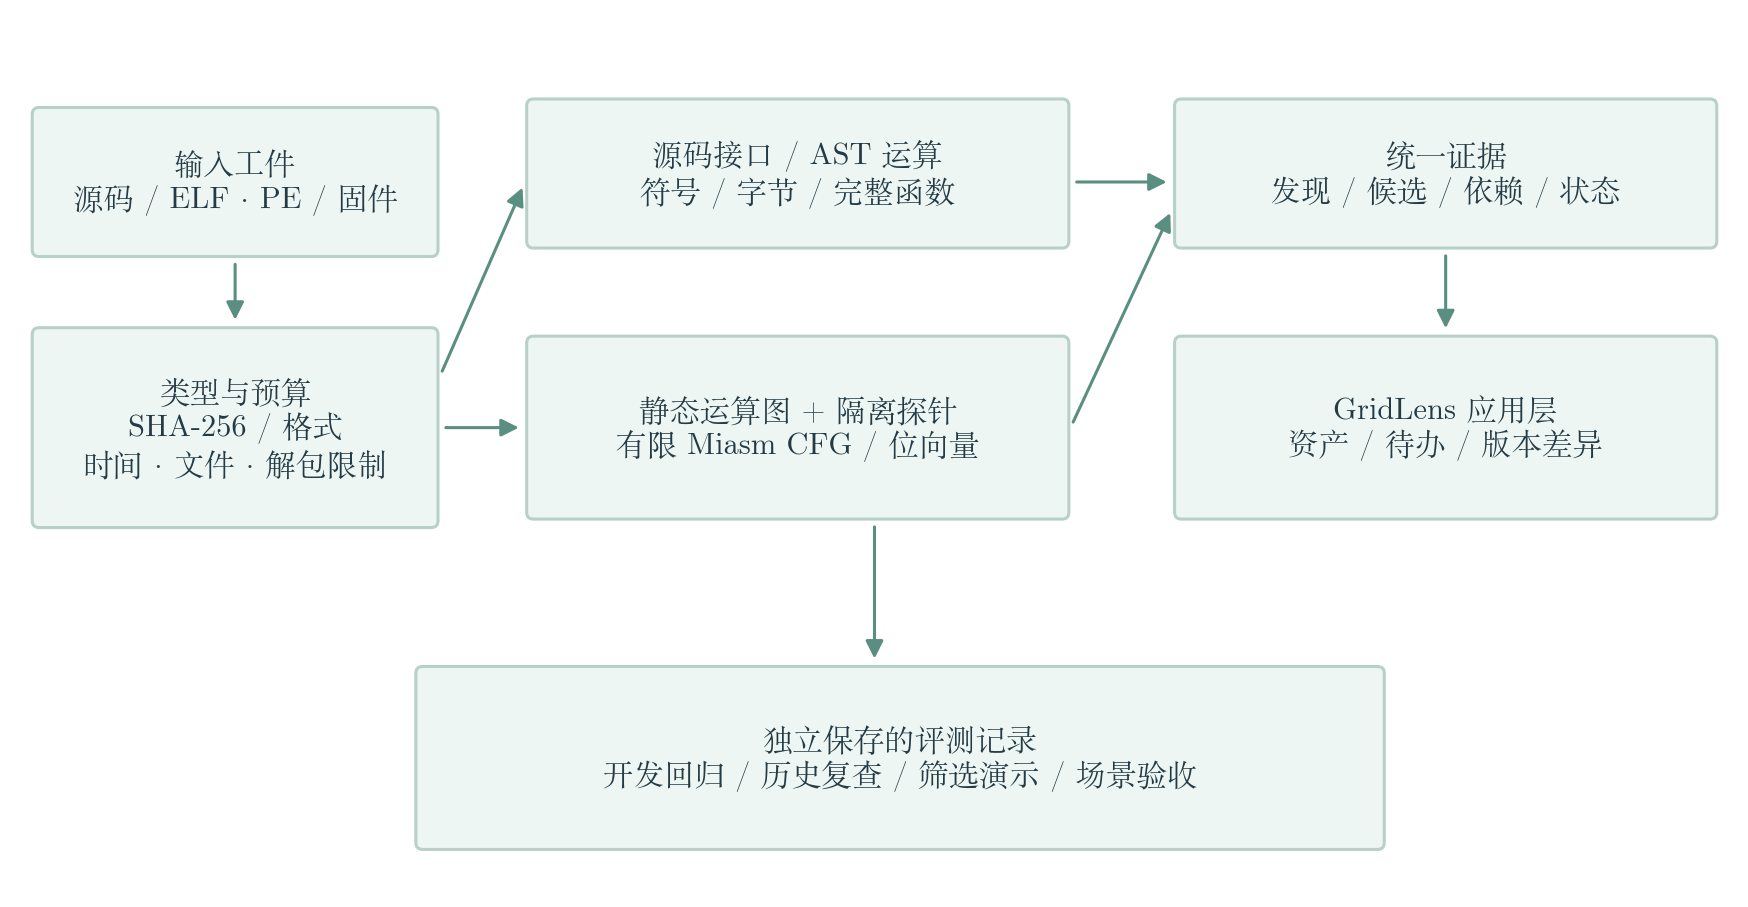
\includegraphics[width=\linewidth]{03-system-architecture.png}
  \caption{当前 QCS 检测引擎、证据模型与 GridLens 应用层。各分析通道按对象与预算适用。}
  \label{fig:qcs-principle-flow}
\end{figure}
% 配图注释（P03）：放一张横向系统架构示意图，区分输入、识别引擎、统一证据和应用层。
%   保留“候选/未知/状态”分支；不要把所有通道画成必定成功的线性流程。

\subsection{源码词法掩盖与接口角色判定}
\label{subsec:source-principle}

源码检测首先解码文本，再对注释和字符串进行词法处理。
当前实现采用严格 UTF-8 解码，失败后尝试严格 CP1252；
它不执行任意编码识别。
若把正则表达式直接应用于原始文件，
注释中的调用示例、字符串中的接口名称与真实调用可能具有相同外观。
因此，工具维护两个等长视图：
代码视图遮盖注释和字面量，
参数视图遮盖注释而保留字面量。
遮盖字符替换为空格，同时保留原始换行和字符位置。
由此可以在去除干扰后，仍将候选定位回原文件的行号。
对于多字节文本，字符位置不应直接等同于二进制字节偏移。

词法器处理行注释、块注释、转义引号、行续接和 C++ 原始字符串，
使 URL 内的双斜线不会错误截断字符串。
工具在代码视图中寻找已审核的精确接口名称，
结合括号与附近的语法形式，将候选分为调用、定义、声明、
宏定义以及名称或类型引用。
明确调用形成静态接口引用；已知算法接口的定义先形成命名依据，
只有源码摘要与已审核参考记录相符时，才形成固定源码实现证据。
另一条源码实现路径由后述语法树运算图及其见证约束支持。
声明、宏文本和普通名称仅形成线索。
例如，注释中的 \nolinkurl{mbedtls_aes_crypt_ecb(...)}
与真实调用使用同一接口名称，但不会获得相同证据角色。

直接选择参数用于补充通用接口的身份。
工具在保留字面量的视图中读取当前表达式的实参，
例如 \nolinkurl{EVP_MD_fetch} 的 \texttt{"SHA256"} 参数，
\nolinkurl{EVP_PKEY_CTX_new_id} 的 \nolinkurl{EVP_PKEY_RSA} 参数，
以及 Mbed TLS 的算法枚举或 \texttt{is224} 参数。
只有直接可见且符合审核规则的参数才参与算法细分。
设接口为 $f$、角色为 $r$、直接选择参数为 $s$，
其身份判定可写为
\begin{equation}
  A=\operatorname{Map}(f,r,s),
  \qquad A\in\mathcal{A}\cup\{\bot\},
  \label{eq:source-identity-map}
\end{equation}
其中 $\mathcal{A}$ 为可记录的算法集合，$\bot$ 表示身份未确定。
同一接口可能具有多算法含义；映射不要求每次返回一个单独算法。

这一接口路径属于词法与局部上下文分析，本身不构建抽象语法树。
独立的源码运算路径使用 Tree-sitter 及有限内部调用关联，
但整体仍没有完整展开预处理器、跟踪任意函数指针或进行全程序数据流分析。
未激活的条件编译分支仍可能被视为源码文本，
变量间接携带的选择器也可能无法恢复。
这些限制随报告说明，避免把源码引用解释成当前构建一定包含或运行的功能。
补充文本扫描得到的关键词和宽泛接口命中仅作为弱线索保存。

\subsection{程序格式解析与符号证据}
\label{subsec:symbol-principle}

结构化符号分析按照程序文件格式读取命名记录，
减少普通字符串、调试文本或文档内容对接口判定的干扰。
ELF 路径同时读取 \nolinkurl{.symtab} 和 \nolinkurl{.dynsym}，
保留符号表来源、地址、位宽和字节序。
符号所属节为 \nolinkurl{SHN_UNDEF} 时记为外部引用；
其余相应定义记为对象内部的命名证据。
来自两个表的同一符号去重后仍保存来源集合，
不会因为在两张表中出现而被计算为两个独立算法。

PE 路径通过命名导入和延迟导入记录接口及 DLL 来源。
只有序号的导入无法直接恢复算法名称，需保持未解析；
当前路径也不等价于全面识别静态链接 PE 内部的密码函数。
ELF 的 \nolinkurl{DT_NEEDED} 则单独形成库依赖。
依赖 \nolinkurl{libcrypto} 只能说明外部库关系，
不能展开为 AES、RSA、ECDSA 等全部算法均存在。

算法映射采用经审核的专用接口集合。
通用大整数、椭圆曲线点运算或通用 EVP 入口，
只支持其共享类别线索。
这使符号通道可以跨处理器读取标准格式，
但具体算法覆盖仍依赖接口命名与符号是否保留。
删除符号后未命中此通道，并不构成算法不存在的证据。

\subsection{字节规则、架构约束与共享特征}
\label{subsec:yara-principle}

YARA 通道对字节序列进行常量、表与机器码模式匹配\cite{yara-docs}。
设文件为 $B$，规则 $R$ 含模式 $p_1,\ldots,p_m$ 和布尔条件 $C_R$，
则原始命中为
\begin{equation}
  \operatorname{Hit}(R,B)
  =C_R\bigl(\operatorname{Match}(p_1,B),\ldots,
             \operatorname{Match}(p_m,B)\bigr).
  \label{eq:yara-raw-hit}
\end{equation}
该式只判断模式组合满足条件，未验证完整的密码运算语义。
整文件条件还可能把不同函数或数据区的模式合并为一次命中。
因此，本工具将原始规则与经过审核的算法含义映射分开管理。
映射记录证据类型、确定身份或候选集合、架构约束、
判别项和解释理由。

某条规则匹配到共享常量时，其候选集合可以表示为
\begin{equation}
  \Gamma(R)=\{a_1,\ldots,a_k\},\qquad k>1.
\end{equation}
共享 SHA-2/BLAKE2 IV、DES 基础表、ChaCha/Salsa 常量
以及 Keccak 置换特征均按这一原则处理。
对于含共享 IV 的 MD5/SHA-1 规则，还检查实际命中是否包含专用判别项。
缺少该项时保留候选，不直接沿用规则名称给出算法身份。
若规则未进入审核映射，记录未映射错误及原始线索，
并将扫描标为不完整。

架构约束在字节命中后再次检查。
x86-64 指令规则只有在程序架构已被结构化解析确认为 x86-64 时，
才按相应指令证据输出；
在其他或未知架构上，相同字节可能代表无关指令或数据，
因此抑制其算法身份。
常量规则具有较少的架构依赖，但仍受字节序、布局和表生成方式影响。
报告保存全部命中偏移、长度、十六进制字节、规则摘要及映射摘要，
便于回溯判定来源。

\subsection{整函数签名与地址变化处理}
\label{subsec:function-principle}

无符号程序缺少接口名称时，
本工具通过已知实现的整函数字节约束补充识别。
参考库选取固定版本的 Mbed TLS、TinyCrypt 和 micro-ecc，
从带符号构建中取得操作函数的边界与算法角色
\cite{mbedtls-source,micro-ecc-source,esp-idf-source}。
识别目标仍是特定参考构建中的已知代码，
而不是从任意大整数或点运算推断密码算法。

同一函数在不同链接布局下，调用地址、相对位移和常量地址可能改变。
直接比较所有字节会将这类变化误作不同实现；
任意放宽指令字节又会丢失计算行为的区分能力。
本工具读取参考可重定位对象中的真实重定位记录，
将对应地址字段转换为逐位掩码，
与链接后函数字节配对。
掩码保留操作码、寄存器、非地址立即数与函数长度。
AArch64 的链接松弛可能将 \texttt{ADRP+ADD} 改写为 \texttt{NOP+ADR}，
建库时按最终指令重新处理其地址字段。
因此，掩码来源是可审计的构建记录，而不是猜测哪些字节可以忽略。

设参考函数字节为 $F=(f_0,\ldots,f_{L-1})$，
掩码为 $M=(m_0,\ldots,m_{L-1})$，
候选目标位置为 $o$。
当掩码位为 1 时要求该位精确一致，
整函数约束为
\begin{equation}
  \operatorname{BodyMatch}(F,M,B,o)
  =\bigwedge_{i=0}^{L-1}
    \bigl(((B_{o+i}\oplus f_i)\land m_i)=0\bigr).
  \label{eq:whole-function-mask}
\end{equation}
候选范围必须完整落在可执行段内，并满足记录的长度与对齐约束；
工具不据此恢复目标程序的全部函数边界。
候选来自目标 ELF 的可执行 \nolinkurl{PT_LOAD} 段，
从而排除仅存放在非可执行数据段中的函数字节拷贝。
它仍不证明相应代码会在业务中执行。

为减少整段逐位置比较，工具选择长度不超过 64 字节、
有效约束位最多的短窗口，用 YARA 先定位候选。
YARA 的十六进制通配只能表达较粗的位约束，
短窗口结果随后按式~\eqref{eq:whole-function-mask} 对全部字节逐位复核。
短锚点独立命中不会产生算法发现，
最终结论取决于完整函数约束。
运行时无需目标函数名，也不依赖完整反汇编或学习模型。

\subsection{只读常量约束与散列角色组合}
\label{subsec:hash-disambiguation}

地址字段被遮盖后，还必须验证目标函数实际引用的数据。
否则，初始化指令形式相同但常量不同的散列变体，
可能满足相同代码掩码。
建库时记录 x86 RIP 相对寻址、AArch64 页相对加载所引用的只读常量；
运行时从目标函数的真实位移恢复地址并核对常量内容。
当前 ARM 参考函数内的常量池保持为精确字节约束。
文件中另放一张未被函数引用的 IV 或轮常量表，不满足这一条件。

若 $\mathcal{L}_F$ 为函数记录的常量约束集合，
完整函数匹配要求
\begin{equation}
  \operatorname{FunctionMatch}
  =\operatorname{BodyMatch}
   \land\bigwedge_{\ell\in\mathcal{L}_F}
       \operatorname{LiteralMatch}(B,o,\ell).
  \label{eq:function-literal-match}
\end{equation}
地址重定位容忍链接布局变化，
常量约束保留算法参数差异，二者共同决定识别范围。

对 SHA-256，还需要同一实现家族的互补函数角色。
设家族 $g$ 的必要角色为 $\mathcal{R}_g$，
已匹配角色集合为 $\mathcal{W}_g$，则
\begin{equation}
  \operatorname{FamilyComplete}(g)
  \iff \mathcal{R}_g\subseteq\mathcal{W}_g.
  \label{eq:family-role-completeness}
\end{equation}
TinyCrypt 使用初始化与最终输出角色，
Mbed TLS 使用初始化与压缩角色。
仅有共享压缩或不完整初始化证据时，输出仍为候选。
角色组合在同一对象与参考家族内核对，
不会将不同库的任意函数拼成新的完整实现。
RSA、ECDSA 和 ECDH 则要求匹配算法操作、签名或协商函数，
不使用通用大数、点乘函数替代这些角色。

当前数据库适用于小端 x86-64、AArch64 和 ARM 模式的链接 ELF。
编译器、版本、优化、配置宏、内联、LTO 与混淆变化均可改变整函数形式。
因此函数签名证据记为中等级别的已知实现证据，
并随之记录参考构建摘要、签名标识、匹配函数及数据库摘要。
未匹配到已知库不能解释为没有非对称算法。

\subsection{固件组件提取与来源可追溯性}
\label{subsec:firmware-principle}

固件镜像可能包含引导头、压缩文件系统与多个程序组件。
当前优先使用经审核的原生 SquashFS、gzip 与受限 ESP 适配器；
SquashFS 通过 \texttt{unsquashfs} 在临时目录中提取文件。
锁定版本的 Binwalk 2 属于可选历史回退，在本文最终环境中不可用，
不能将其写成这一环境已经成功运行的必要依赖。
解包后逐文件检查类型，再调用已有源码、程序或固件入口。
工具不执行下载的目标程序，
但提取过程会运行外部解包器；临时目录和资源限制不等价于完整安全沙箱。

固件内证据通过镜像摘要、组件摘要、文件系统内路径与解包链关联。
普通文件摘要为内容 SHA-256；
目录摘要则由排序路径和组件摘要组合，二者含义分别记录。
嵌套镜像使用 \texttt{!/} 连接逻辑路径，
报告中的稳定组件标识由外层镜像摘要和逻辑路径构成，
避免把已删除的临时绝对路径作为资产位置。
只有能明确对应时才保存文件系统镜像偏移；
多个文件系统无法对应时保持空值。
压缩文件中的解压后偏移也不能直接当作外层固件字节偏移。

组件扫描不跟随符号链接，
目录遍历和嵌套提取共享文件数、总字节、递归深度与时间预算。
达到限制时保留已经取得的证据，并明确未处理部分。
原生适配器覆盖之外的容器、加密区域和不可解析镜像，
记录为不支持或失败，而不返回虚假的完整阴性报告。

\subsection{证据归一化、资产汇总与完成状态}
\label{subsec:report-principle}

每条证据保存算法、类别、引擎、标识、行号或偏移、
置信等级及理由，并附带通道特有信息。
本工具将能够支持明确算法身份的静态证据放入发现集合，
将共享候选、编码特征与宽泛名称放入线索集合，
库依赖和错误独立记录。
这种组织保留证据的原始含义，
不会通过多条弱线索投票把共享结构自动升级为确定身份。

设算法 $a$ 的发现证据集合为 $E_a$，
资产汇总保留全部 $E_a$，并按
$\mathrm{low}<\mathrm{medium}<\mathrm{high}$ 的序关系取最高等级：
\begin{equation}
  c(a)=\max_{e\in E_a}c(e).
\end{equation}
这一等级表示规则依据的相对强弱，
没有通过校准转换为正确概率。
多条规则命中同一算法时，仍只形成一个规范算法资产，
但具体证据及组件归属继续保留。
固件顶层汇总递归收集组件发现，因此顶层局部发现列表为空
不表示整幅镜像没有算法资产。

扫描状态区分流程是否完成与算法是否识别正确，见表~\ref{tab:qcs-status}。
已取得有效结果但存在错误、受限通道或未支持组件时，通常归为部分完成；
没有有效通道且发生错误时归为失败。
有意关闭或不适用的通道单独标为停用，不必然令其他成功通道失败。
缺失依赖、规则编译失败和超时均保留错误信息，
不会被静默转换为空发现。

\begin{table}[htbp]
  \centering\small
  \caption{扫描状态的含义及命令行退出码}
  \label{tab:qcs-status}
  \begin{tabularx}{\linewidth}{l c X}
    \toprule
    状态 & 退出码 & 解释\\
    \midrule
    \texttt{completed} & 0 & 支持范围内的步骤完成；不代表算法不存在或识别全部正确。\\
    \texttt{partial} & 2 & 已保留部分结果，但存在限制、失败通道或未支持组件。\\
    \texttt{unsupported} & 3 & 当前无法按指定方式分析该对象。\\
    \texttt{failed} & 4 & 输入或必要处理失败，不能获得相应完整结果。\\
    \bottomrule
  \end{tabularx}
\end{table}

\subsection{资源控制与双口径评测的联系}

扫描器默认使用 60 秒时间预算、10000 个文件、4 层固件递归、
1 GiB 总字节与 256 MiB 单文件限制。
外部提取进程在超过预算时终止其进程组，
组件分析也继续沿用同一预算对象。
这些机制减少失控遍历和过量提取，但依赖周期性监测，
不能宣称为严格的实时内核限额。

报告中的证据角色直接决定评测口径。
源码明确调用与二进制导入进入接口引用集合；
与固定参考摘要相符的源码实现、带标准依赖见证的源码运算图、
已定义符号、审核后的常量/指令和整函数签名进入实现包含集合。
单纯源码命名定义不进入该集合。
共享候选不进入任何确定预测集合。
两种集合分别与预先标注的真值比较，
因此工具可以区分“引用了外部接口”和“对象内含实现”的检测效果。
第三章给出样本构建、真值审核、执行命令和指标计算方案，
第四章按这些约定给出已经完成的实验结果和未完成事项。

\section{运算语义、有限控制流与原语摘要}
\subsection{从代码特征到带数据依赖的运算见证}
后续版本增加源码语法树、指令解码、局部表达式与静态调用关系，
使识别不完全依赖函数名或单个字节序列。
例如，SHA-256 的轮计算需要关联 $\mathrm{Ch}$、$\mathrm{Maj}$、
大/小 $\Sigma$、消息调度、实际使用的轮常量和 SHA-256 IV；
共享 SHA-224 压缩结构不能单独确认 SHA-256。
SM4 需要关联表查找、特定线性变换、轮密钥与反馈，
公钥识别需要满足已实现的模运算或曲线协议关系。
源码侧有限关联局部头文件、数组初始化和内部调用，
但没有替代编译器完整的预处理、类型系统与全程序分析。

对加法、异或和旋转作正规化时保留输入身份与字宽。
例如同一 32 位值的左右移位可合并为旋转，
结合律加法可以展平，低 32 位截断只对相容的运算下推。
若把不同分支或无关输入上的旋转混合统计，可能得到假的轮结构；
因此算法见证由同一有界依赖图支持，而非仅由运算出现次数支持。

\subsection{Miasm 的进程隔离与有限 CFG}
Miasm 将机器指令提升为中间表示，再执行符号状态传播\cite{miasm}。
自写控制器验证请求、选择固定外部解释器、限制资源，并以 JSON 交换结果。
原生指令与指令内部 IR 块都进入有界工作队列。
相对分支先正规化为地址标签，寄存器别名和零扩展由提升语义处理。
当前有限直接 CFG 主要覆盖 x86-64、ARM、Thumb 与 AArch64；
MIPS 大小端可处理其已支持直线片段，延迟槽控制转移是显式边界。
调用、间接边及 Thumb IT 等未完整处理时保留部分状态，而不推断完整出口语义。

令状态映射 $S$ 为寄存器或可确认位置到表达式的映射，
两路径合并采用相同事实保留策略：
\begin{equation}
 (S_1\sqcup S_2)(x)=
 \begin{cases}
 S_1(x),&S_1(x)=S_2(x),\\
 \mathrm{unknown}_{x,w},&\text{否则}.
 \end{cases}
\end{equation}
其中 unknown 具有稳定身份和位宽 $w$。
循环中冲突值扩大为 unknown，以推动保守收敛；
该方法不证明全部路径可达性，也不是 SMT 驱动的完整路径求解。
内存写可能与既有事实别名，因而保守清除旧内存事实，
只保留可确认的最新精确地址写后读。
预算耗尽且未收敛时不输出临时表达式作为完整摘要。

\subsection{带位宽、输入身份与来源的摘要}
位向量加法写为
\begin{equation}
 z=\operatorname{add}_w(x,y)=(x+y)\bmod 2^w.
\end{equation}
同一宽乘在 32 位和 64 位语义下具有不同截断和高位输出，不能丢弃位宽。
摘要包含表达式标识、操作数引用、输入身份、位宽、地址范围、代码摘要及覆盖说明。
进位、借位和宽乘可记录为原语，但其字段为
\nolinkurl{primitive_only=true}、\nolinkurl{algorithm_eligible=false}。
这些记录不自动等价于 Montgomery 约减、模幂、模逆或曲线协议。
当前生产桥接主要消费合并后的寄存器出口表达式，
独立 API 可返回的内存结果尚未完整接入算法消费。

后端每次限制 256 条原生指令、512 个 IR 块、1024 个 IR 步和 32768 个表达式节点，
地址空间上限 512 MiB、输出上限 512 KiB；
摘要还限制至多 64 个不同运算公式、4096 个公式节点。
这些上限是工程预算，不意味着分析范围恰好覆盖一个完整函数。

\subsection{原语与算法的桥接边界}
已有识别器可以从满足依赖条件的 32 位表达式恢复 ChaCha 四分之一轮：
\begin{align}
 a&\leftarrow a+b,&d&\leftarrow\operatorname{ROTL}_{32}(d\oplus a,16),\\
 c&\leftarrow c+d,&b&\leftarrow\operatorname{ROTL}_{32}(b\oplus c,12),\\
 a&\leftarrow a+b,&d&\leftarrow\operatorname{ROTL}_{32}(d\oplus a,8),\\
 c&\leftarrow c+d,&b&\leftarrow\operatorname{ROTL}_{32}(b\oplus c,7).
\end{align}
四个输入的身份和更新次序是依据的一部分；
单独出现 16、12、8、7 四个常量不构成等价证据。
这一桥接通过针对性正反例，不代表后端已在未知生产实现中新增检出。
RSA 与曲线算法仍需 ABI、输出缓冲区、调用副作用和完整协议方程的进一步约束。
二进制通常丢失源变量名、类型和宏信息，提升 IR 或生成伪代码不等于恢复原始源码。

\section{从识别证据到迁移待办的原理}
GridLens 将资产按“文件、算法、证据范围”合并，保留核心证据与原始报告入口。
业务模块来自显式场景清单，风险类别来自可审查规则：
MD5/SHA-1 等进入遗留用途复核，传统公钥接口进入量子迁移关注，
其他对称和摘要资产进入模式、密钥或用途复核。
动态提供者调用而算法参数未知时单列覆盖待确认，不计成具体算法资产。
迁移任务引用相应资产或文件，人工状态独立存储，不能反向修改算法发现。

% 配图 P04：真实源码证据弹窗，需看清输入哈希、行号、MD5 调用和原始报告入口。
\begin{figure}[htbp]\centering
  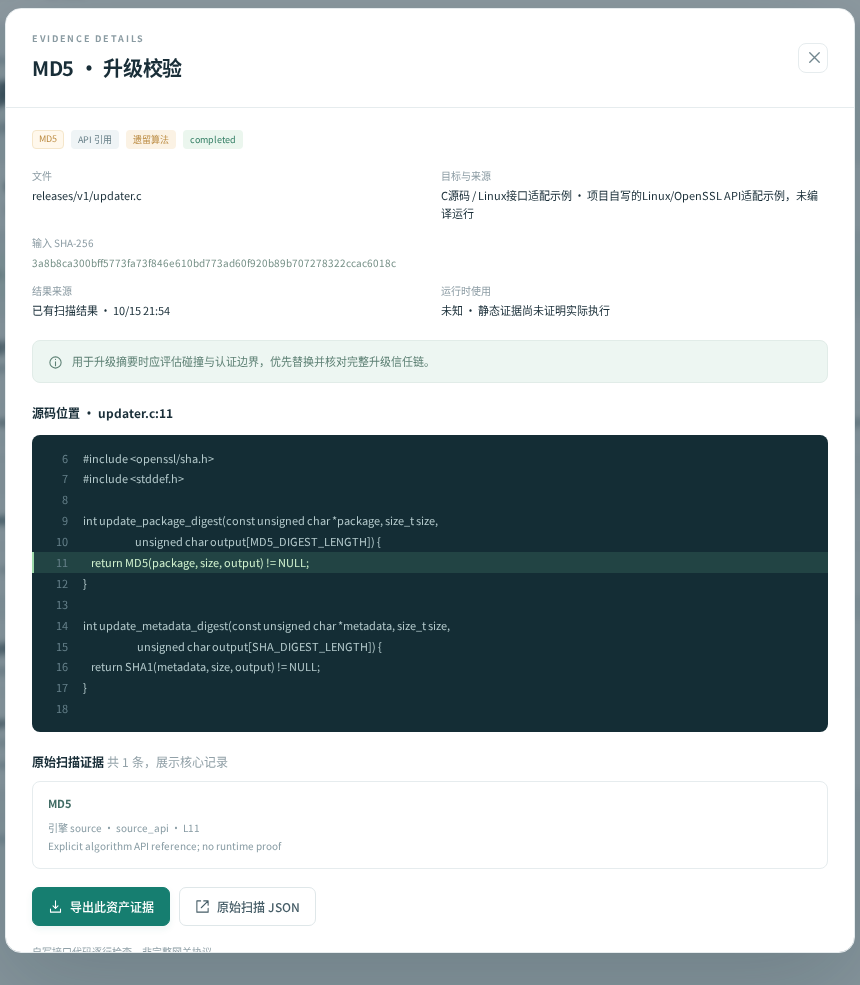
\includegraphics[width=.82\linewidth,height=.72\textheight,keepaspectratio]{04-source-evidence.png}
  \caption{GridLens 展示真实源码扫描证据。高亮行、输入哈希及原始报告入口构成可审查链。}
  \label{fig:source-evidence}
\end{figure}
% 配图注释（P04）：放界面局部截图而非流程图：保留 MD5 调用高亮、文件路径、SHA-256 与证据类型。
%   截图只裁去无关页边，不更改扫描数字；避免缩到无法阅读源码。
